\chapter{Methodology}

\section{\label{data_collection}Data Collection}

    When mining Github and Stack Overflow, a natural starting point is to use GHTorrent \cite{gousios2013ghtorent} and SOTorrent \cite{baltes2018sotorrent} as data sources.
    \subsection{Stack Overflow data}
        SOTorrent\footnote{\label{SOTorrent}\url{https://empirical-software.engineering/projects/sotorrent/}} is an open data set based on periodic, official Stack Overflow data dumps. SOTorrent was built for the purposes of mining and analyzing the evolution of Stack Overflow posts. A new version of this data set based on the latest Stack Overflow data dump is released every 3 months. Each version of the SOTorrent datas set can be downloaded from Zenodo\footnote{\label{SOTorrent_Zenodo} \url{https://zenodo.org/record/2273117}}. The latest versions of the SOTorrent data set are also available online, and can be queried through Google BigQuery\footnote{\label{BigQuery} \url{https://bigquery.cloud.google.com/dataset/sotorrent-org:2018_12_09}}.
        
        When downloading the SOTorrent data set, the version from \textit{December 9th 2018} was used, as it was the latest version available at the start of the project. The SOTorrent data set has its files organized into tables. Not all tables were downloaded, as certain tables related to post evolution (e.g. PostHistory, PostVersion tables) were deemed to be unrelated to the expertise learning task. The tables downloaded included Users, Posts, PostLinks, PostType, PostReferenceGH, Comments, CommentUrl, GHMatches, Tags, Badges and Votes, totaling 29 GB of compressed raw data. After downloading and un-compressing all relevant data files, the data set contained just shy of 100 GB of data.
        
    \subsection{Github data}
        GHTorrent\footnote{\label{GHTOrrent}\url{http://ghtorrent.org/}} is also an open data set, which mirrors the data offered through the Github REST API\footnote{\url{https://developer.github.com/}}. GHTorrent has been collecting data from all public projects available on Github and releases a new version of MySQL data dumps every month, while it also offers daily data dumps through MongoDB. Each version of MySQL data can be downloaded from GHTorrent\footnote{\label{GH_dowload}\url{http://ghtorrent.org/downloads.html}}. GHTorrent data can also be looked at and queried online, as it is available as a DBLite web interface\footnote{\label{GH_query}\url{http://ghtorrent.org/dblite/}}. 
            
        When downloading the GHTorrent data set, the version from \textit{March 1st 2019} was used, as it was the latest version available at the time of download. The data set has its files organized into large tables stored in compressed CSV files, totaling 96557 MB of compressed data. All files were downloaded and uncompressed which resulted in 21 raw data tables totaling over 400 GB of data.

\section{Data Storage}

    \subsection{Database Setup and Data Import}

        
        A MySQL database was the obvious choice of database, as both data sources come with SQL scripts performing table creations, data imports and general database manipulations\footnote{\label{SO_sql} \url{https://github.com/sotorrent/db-scripts/tree/master/sotorrent}} \footnote{\label{GH_sql} \url{https://github.com/gousiosg/github-mirror/tree/master/sql}}. Managing disk space during the data import phase represented a challenge, as the raw, uncompressed data files totaled up to over 500 GB. Importing of the data into the database was not achieved all at once, but rather through several iterations of uncompressing only a few data files. After a file was uncompressed and the table was successfully imported into the database, its raw CSV or XML file was deleted to free up disk space. 
        
        During the data import phase it was discovered that using \textit{MyISAM} over \textit{InnoDB} as the database engine is more favorable, since there was a significant execution time difference between the two database engines when importing large amounts of data into the MySQL database. \textit{MyISAM} database engine does not support foreign keys constraints, while it supports table-level locking. On the other hand \textit{InnoDB} supports foreign key constraints and row-level locking. \textit{MyISAM} is preferred when performing tasks that require fast import and querying speed, while \textit{InnoDB} being the default database engine for MySQL is more optimal for regular operations. For this particular reason all of the large raw data files were imported into the database using the \textit{MyISAM} database engine. After all necessary database manipulations have been performed, the database engine was changed back to the default engine, \textit{InnoDB}, to allow foreign key constraints to be enforced. 
     
        \todo{Add table contains descriptions for each relation's content}
      
        \begin{figure*}[!h]
          \centering
          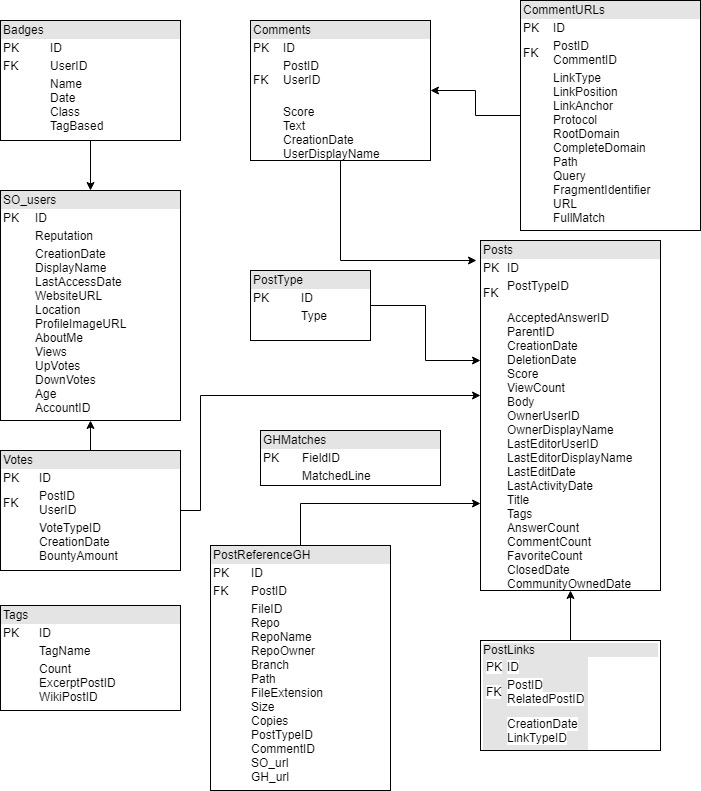
\includegraphics[width=0.9\textwidth]{SO_DB_schema.jpg}\\
          %\caption{Redesigned database schema for the downloaded Stack Overflow data.}
          \label{fig:so_schema}
        \end{figure*}
        
   
        \todo{Re-do this image}
        \begin{figure*}[!h]
          \centering
          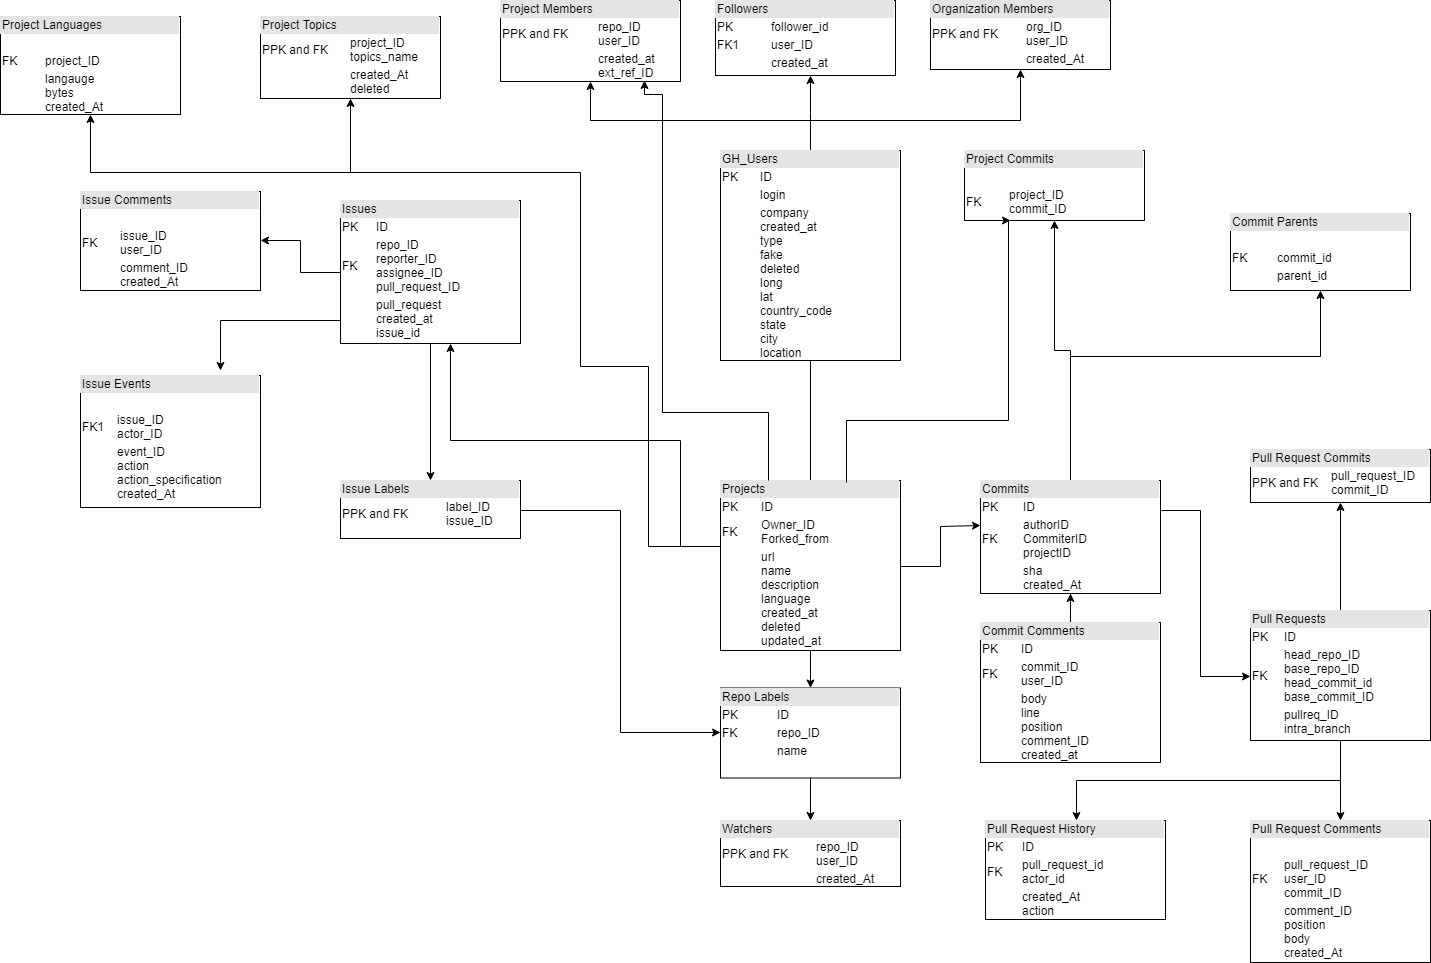
\includegraphics[width=\textwidth]{GH_DB_schema.jpg}\\
          %\caption{Redesigned database schema for the downloaded Github data.}
          \label{fig:gh_schema}
        \end{figure*}
        
        Figure \ref{fig:so_schema} and \ref{fig:gh_schema} show the database schema and all attributes within each table of the SOTorrent and respectively the GHTorrent data set. All tables from GHTorrent are shown in figure \ref{fig:gh_schema}, while only the relevant tables from SOTorrent are shown in figure \ref{fig:so_schema}. 


    \subsection{Linking together GHTorrent and SOTorrent}\label{Linking_SO_GH}
    
        In order to perform cross platform analysis of Github and StackOverflow, the linking of GHTorrent and SOTorrent datasets is needed. This task requires identifying the same user's accounts on both platforms. Looking at relevant literature on this this problem, one can identify the task of \textit{identity merging}, which consists of identifying the same person in two or more different environments. Vasilescu et al. \cite{vasilescu2013stackoverflow} researched this problem rigorously and after careful consideration of limiting the number of false positives they made use of email addresses. In 2013, at the time of publishing their work, email addresses were present in the Github dataset, while in the StackOverflow dataset email addresses were hidden, but their MD5 hashes were available. Vasilescu et al. \cite{vasilescu2013stackoverflow} decided to ``merge (i.e., link) a GitHub and a Stack Overflow user if the computed MD5 hash [of the email in Github] is identical to the MD5 email hash [of Stack Overflow users]". This resulted in 93,771 GitHub users being linked to StackOverflow. Vasilescu et al. \cite{vasilescu2013stackoverflow} further investigated, and came to the conclusion that out of 93,771 linked users only 46,967 users were active at the time. The linked data set alongside a replication package has been made public by the authors of the paper\footnote{\label{bodgan_dataset}\url{https://www.win.tue.nl/mdse/stackoverflow/}}. This data set has been used multiples times to analyze the interaction of Github and Stack Overflow data \cite{badashian2014involvement} and \cite{lee2017github}, thus it became the backbone of the data sampling process behind linking together Github and Stack Overflow users.  

        There was one major problem with using Vasilescu et al. \cite{vasilescu2013stackoverflow}'s data set. The replication package contained a data set linking Github email addresses to Stack Overflow user IDs, without fully mapping Github user IDs to Stack Overflow user IDs, therefore the mapping of Github email addresses to user IDs was needed. This mapping was possible when Vasilescu et al. \cite{vasilescu2013stackoverflow} published their work, but after March 2016 GHTorrent was not allowed to store email addresses in their open data sets, as it violated GDPR compliances. The solution to this problem was to download the \textit{User} table data from GHTorrent's last available version that still contains email addresses of Github users in the data set. This older version of GHTorrent is dated \textit{February 1st 2016}, and it was downloaded, then imported into the MySQL database. A manual check was performed on matching user IDs and login names between the \textit{User} table's March 2019 and February 2016 versions. This manual check made sure that the user IDs from both versions of the table are referring to the same login name. If this was not the case, the user was dropped from the data set, due to inconsistency of the two versions of table. This manual check assured consistency in the data linkage between Stack Overflow and Github users, but resulted in the removal of over 10,000 users from the original 93,771 users linked. The final data set contains 83,550 user accounts being linked between the two platforms, offering a unique Github user ID to Stack Overflow user ID mapping. It can be speculated that removed users either deleted or changed the login name of their Github account between 2016 and 2019, thus causing the inconsistency in the two versions of the \textit{User} table.
        
    \subsection{Discarding Unlinked Data}
       As mentioned in section \ref{data_collection}, the total size of the GHTorrent data set was over 400 GB of data, while SOTorrent contained close to 100 GB of data. In order to make data querying and processing more efficient, the reduction the full data set was desired. In order to perform analysis only on the linkage between Github and Stack Overflow, only successfully linked data is needed. Filtering out unlinked data was done by iterating through each existing table in the database and keeping only the observations that are connected or related to users with a user ID present in the list of 83,550 unique user IDs linked. Discarding unlinked data reduced the size of the data set and allowed only linked data to be analyzed. This process reduced the size of the MySQL database from over 500 GB of data to 122 GB.
        
\section{Data Aggregation} 
    The end goal of the analysis on Stack Overflow and Github data was to create topic models capable of deciphering the hidden patterns of underlying topics that represent a user's activity on a platform. Tian et al. \cite{tian2013predicting} modeled user topical interest and expertise by building LDA models on user activity data. The authors have showed that a Stack Overflow user's expertise can be extracted using a topic model applied over a set of textual documents consisting of the user's activity on the platform. 

    In order to perform cross platform analysis of Github and Stack Overflow users' expertise, the modeling of their expertise through LDA models is needed. LDA topic models are fit on a set of documents. In order to fit LDA models on Github and StackOverflow user data, one needs to define what a document consists of, and how to extract a user profile from a platform such as Github or Stack Overflow.  
    
    \subsection{Extracting Stack Overflow User Profiles}
        When deciding how to create documents for the LDA topic model, the simplest approach was to start by defining a document as a user profile. Each user present in the data set of 83,550 linked users described in section \ref{Linking_SO_GH} has one document (user profile) describing their activity on StackOverflow.
    
    \subsection{Extracting Github User Profiles}
    
    \subsection{Creating Time Based User Profiles}
    After defining how to extract user profiles from both Stack Overflow and Github, it is worth factoring in a \textit{timeline} into the user profile. The simplest approach would be to model recent and past activity of users by splitting their activity into before and after a specific date. Being able to model past and recent user profile data separately creates opportunities for comparison analyses to be done on the evolution of expertise of Github and Stack Overflow users. A decision was made to define recent activity as the activity performed by a user in the last 3 years. 2019 being the year that this analysis has taken part, the split between past and recent activity was created by any user profile data being dated before or after \textit{January 1st 2016}.
    % deciding how to structure the data for the analysis

\section{Data Cleaning}
Textual data on Stack Overflow and Github contains a large variety of software engineering related domain specific wording mixed with source code. Stack Overflow posts contain rich software artifacts such as code snippets, text blocks explaining problems and solutions using text and source code, comments which can be associated with a question or an answer, and hyperlinks to references such as API documentation or an academic paper explaining an answer. In their study of Github data, Liao et al. \cite{liao2019status} mentions that developers on Github ``talk about project bugs, enhancements, and tasks in issue discussions". The authors stated that a text corpus built on Github data will most likely contain ``plenty of code, warnings, messages, and technical terminology in addition to more general natural language [...] which allow for easy detection of status and/or relevant expertise".

One can conclude that textual data on both Github and Stack Overflow captures a variety of aspects of software development, but its technical terminologies, mix of text and source code makes it difficult to extract the proper textual data to be analyzed. When performing text pre-processing on both sources of data, one needs to find the right balance between more than a dozen pre-processing techniques in order to clean up the data just the right way, without removing software engineering domain specific words and damaging the contextual details of software artifacts. Deciding on a precise set of techniques for the pre-processing routine was a challenging task, thus extensive research was done on what text pre-processing techniques were previously used when analyzing Github and Stack Overflow data.

Tian et al. \cite{tian2013predicting} pre-processed textual data by performing tokenization, stop-word removal and stemming. They also split function names from cleaned up source code related keywords in the text processing phase.

Campbell et al. \cite{campbell2015latent} mentions in a book chapter on extracting topics from software engineering data that generally those who use LDA apply the following pre-processing steps: ``loading text, mapping text into final textual representation, [perform] lexical analysis of the text, optionally removing stop words, optionally stemming, building a vocabulary, optionally removing uncommon or very common words and mapping each text document into a word-bag".

Treude and Wagner \cite{treude2019predicting} have performed similar, but separate pre-processing routines on StackOverflow and Github data. Their Stack Overflow data cleaning routine consisted of removing line breaks, code blocks, all HTML tags, replacing HTML symbols and strings indicating special characters with their corresponding character, and replacing sequences of whitespace with a single space. Their Github pre-processing routine is the same as the above Stack Overflow data cleaning routine, with a few extra steps, such as removing vertical and horizontal lines, code comments, characters denoting sections headers, characters that indicate formatting or links. 

Efstathiou et al. \cite{efstathiou2018word} converted text from Stack Overflow into lowercase, removed code snippets and HTML tags, then performed a ``conservative punctuation removal, keeping symbols that often appear in programming commands, such as ‘+’ and ‘\#’ which are essential for differentiating ‘C’, ‘C++’, and ‘C\#’ from one another."

Boyd-Graber et al. \cite{boyd2014care}'s book chapter recommends HTML symbol and  stopword removal, then normalizing strings by converting to lower case and applying any kind of stemming algorithm, then apply tokenization and any kind of phrase detection algorithm as the proper pre-processing routine before fitting topic models on textual data.

Liao et al. \cite{liao2019status} analyzed issue discussions on Github, and in their pre-processing steps they filtered out code-specific language, which was enclosed in HTML tags. The authors then removed short posts contained less than five tokens and distinguished between data generated by developers who never committed code to a project, and those who did. 




%% user-level: tokenization, html links, symbols, tags, stop-word removal, numeric and punctuation removal (if not part of a word)
%% corpus-level: tokenization, bi-trigram phrase detection (frequency of min 20 for bigrams, min 50 for trigrams)
%% corpus-level: Remove rare and common tokens: Filter out words that occur less than 20 documents, or more than 50\% of the documents
    

\section{Topic Modeling}
    
    \subsection{Experiment Setup}
    %% Creating SO-full and GH-full after inactive user issues
    
    \subsection{Hyper-parameter optimization}
    
    \subsection{Evaluation of model}
    
    \section{Expertise survey}
        \subsection{Survey setup}
        %% task, sampling, who did it
        \subsection{Annotations Cleaning}
        \subsection{Limitations}
        % aggregating the data, (union and intersect)
        
\section{Data Analysis and Algorithm Design}
    %%for each technique
        %% what it is, where do you use it
    
    \subsection{Extracting/ Determining/ Defining Expertise}
    
        %% mean_BLEU_score, mean_Jaccard_sim, Mean_Cos_sim
        \subsubsection{Topic Distribution based Expertise}
        %%% (mention Lda2vec and ETM as alternatives)
        
        \subsubsection{User and Topic Embeddings}
        %%% Avg and Max LDA Emb
        %%% Avg and Max word2vec Emb
        
        %%% k-means, then thresholding
        
    \subsection{Cross-platform expertise}
    %% RQ2 - quantitative diff - distr. of overlap or Jaccard sim.
    \subsection{Cross-platform Knowledge Transfer}
    %% RQ3 - most frequent words used in both platforms
    \subsection{Expertise Evolution}
%% RQ4 - changed ratio or Jaccard dist.

\section{Software Tools Used}



    
